\section{The Plasmasphere}
\label{section:plasmasphere_models}
The plasmasphere is a region of the space environment surrounding the Earth, and a primary unknown within our modeling. The plasmasphere extends from the upper edge of the ionosphere (an altitude of $\sim$ 1000 km) up to several Earth radii; typically it is divided into two separate regions: a dense, relatively cold \emph{inner plasmasphere}, and a sparse, relatively hot \emph{outer plasmasphere} or \emph{trough}. The transition boundary between the two regions is a sharp dropoff in plasma density called the \emph{plasmapause}. The location of the plasmapause varies with magnetic local time (MLT) and solar activity conditions, but generally occurs between 4 $<$ L $<$ 7. Forcing on the sun side tends to bring the location closer to the Earth. Figure \ref{fig:Kp_dist} shows a distribution of \kp{} values. Figure \ref{fig:plasmapause} shows the modeled location of the plasmapause as a function of \kp{}, a measurement of space weather activity. \kp{} is computed on a 3-hour period using ground-based measurements of local deviations from the background magnetic field. \kp{} can range from 0 (very quiet conditions) to 9 (extremely active conditions). Typically \kp{} is around 1 or 2. 

\begin{figure}[h]
\begin{center}
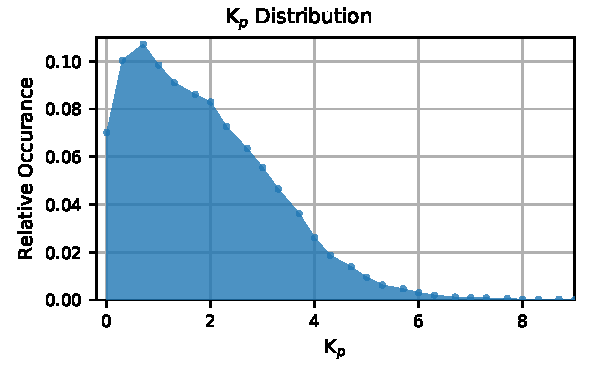
\includegraphics{figures/Kp_distribution.pdf}
\caption[Histogram of \kp{} data]{A histogram of \kp{} values, over a 5-year period between 2012 and 2017.}
\label{fig:Kp_dist}
\end{center}
\end{figure}

\begin{figure}[h]
\begin{center}
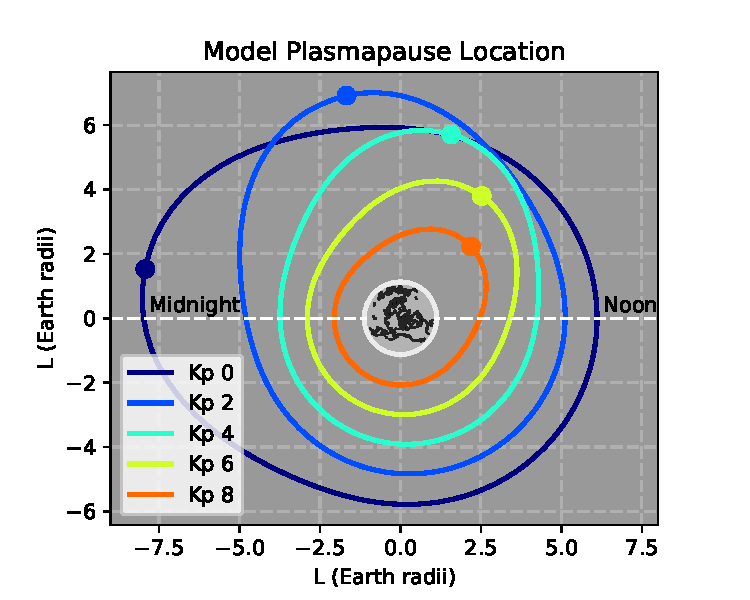
\includegraphics{figures/plasmapause}
\caption[Model of plasmapause location]{The \cite{Gallagher1999} model of the plasmapause location, as a function of \kp{} and magnetic local time. Solid dots indicate the point of maximum extent.}
\label{fig:plasmapause}
\end{center}
\end{figure}


Much like the ionosphere, the plasmasphere is a highly variable region, depending on geomagnetic conditions (\kp{}), location (latitude, longitude, field line), and time of day (MLT). The large spatial scales, high variability, and sparse availability of in-situ measurements require us to turn to empirical models of each region. We consider three primary models of electron and ion density.

\subsubsection{Overview of Plasmasphere Density Models}
\label{section:plasmasphere_density_models}
\paragraph{Ngo Model}

The Ngo model is a legacy model used extensively in research at Stanford from the early 1980s through the mid-2000s, notably by \cite{Lauben1998} and \cite{Bortnik2005}, and has heritage dating back to the early days of radioscience at Stanford \citep{Kimura1966}. The model uses a Diffusive Equilibrium \citep[DE;][]{Angerami1964} model for the inner and outer plasmasphere, onto which the \cite{Carpenter1992} inner plasmasphere model is overlaid. This model was integrated into the legacy Stanford VLF raytracing code, and provided several adjustable parameters, including plasmapause location, constituent ratios, and the ability to include ducts.

\paragraph{Global Core Plasmasphere Model (GCPM)}
\label{section:gcpm}
The Global Core Plasmasphere Model, initially developed in 2000 by \cite{Gallagher1999} with significant updates through the following decade, smoothly transitions between several regional models to provide a continuous model of the plasmasphere. Within this work we use version~2.4, which was released in 2009 and made available by the Space Plasma Physics group at the NASA Marshall Space Flight Center\footnote{Available at \emph{https://plasmasphere.nasa.gov}}. GCPM incorporates the \cite{Carpenter1992} inner plasmasphere model and the \cite{Gallagher1995} outer plasmasphere model, with an empirical fit of the plasmapause location between. The polar cap model is derived from \cite{Persoon1983} and \cite{Chandler1991}. All models are connected smoothly to the IRI model of the ionosphere at lower altitudes. The combined GCPM model is parameterized by \kp{} and MLT.

\paragraph{Simplified GCPM}

GCPM aims to provide a dynamic, complete picture of the plasmasphere as a function of time, location, and \kp{}; however for our purposes GCPM provides much more detail than we require. Additionally, the combination and smoothing between many models is computationally slow. In order to provide quicker computation and to reduce the number of parameters to adjust, we have implemented a simplified version of GCPM.

This model uses the equatorial-plane GCPM model, including the plasmapause location. However we omit any variation in electron density along latitude, and assume densities are constant along each field line. As our region of interest lies primarily within low and mid latitudes, we omit the polar cap model altogether and simply merge the ionosphere into the equatorial trough model. Finally, to simplify computation, we model the ionosphere using an empirical fit to IRI -- one for noon, and one for midnight, with a smooth transition along longitude. Figure \ref{fig:plasma_model_comparison} shows a side-by-side comparison of the three models, for \kp{}$=2$.
\begin{figure}[h]
\begin{center}
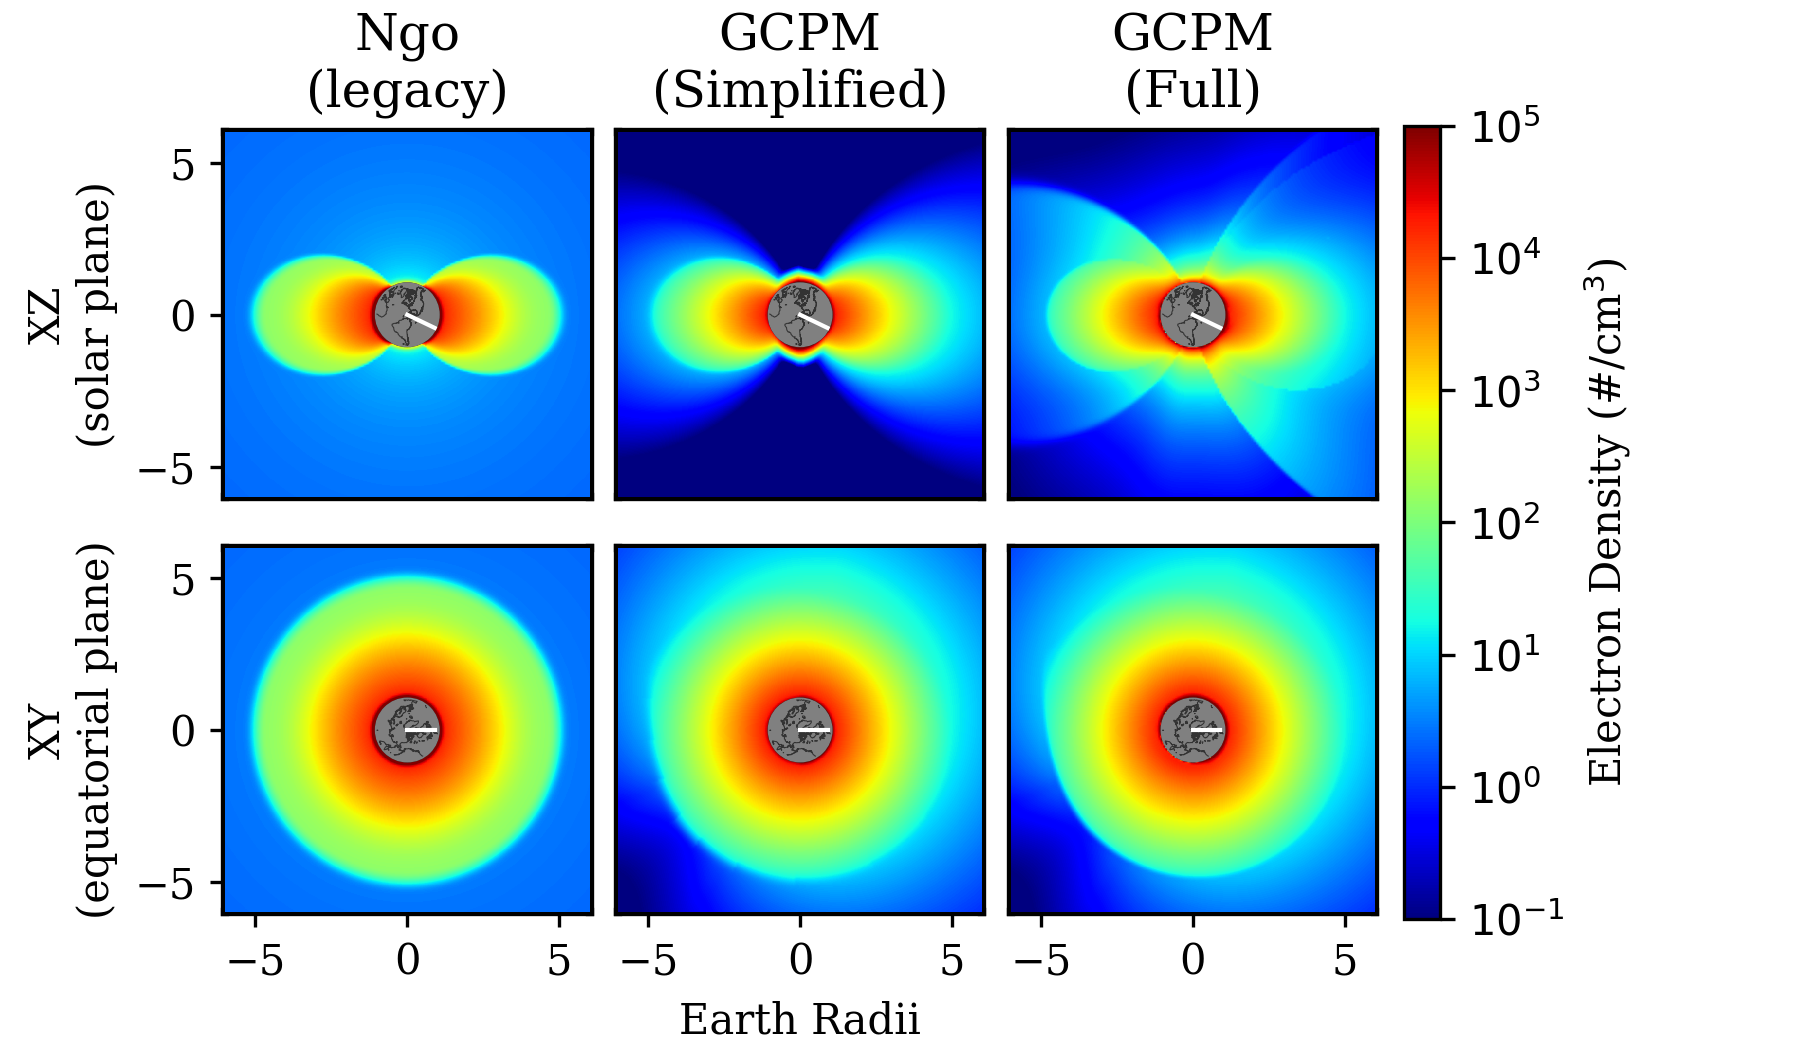
\includegraphics{figures/plasma_model_comparison_serif.png}
\caption[A Comparison of three plasmasphere electron density models]{A comparison of three plasmasphere models: Ngo, simplified GCPM, and full GCPM, for a relatively quiet plasmasphere (\kp{}$=2$). The top row shows electron density in-plane with the direction of solar influx; the bottom row shows a top down (equatorial cross-section) view. The white line indicates the solar axis. Only electron density is shown, as additional plasma constituents are derived from electron density.}
\label{fig:plasma_model_comparison}
\end{center}
\end{figure}


\section{Ray Tracing and Landau Damping}
\label{section:raytracing}
\subsection{Ray Tracing}
Whistler-mode waves in the magnetosphere propagate for very large distances, and with relatively little attenuation. Under certain conditions, these waves can persist from a few seconds to 1 or more minutes. Simulating the propagation of these waves using a full-wave method would be extremely intractable with current computational resources. However we can use ray tracing to approximate their behavior.

Ray tracing is a technique from geometric optics which tracks the position and velocity of a coherent wave packet -- essentially, approximate the behavior of a wave packet to that of a photon, and evaluate the packet's velocity and wavenormal vector with respect to time. Ray tracing is best suited for coherent, monochromatic wave packets, with no attenuation, dispersion, or mode coupling. 

Ray tracing was first applied to the Whistler mode by \cite{Haselgrove1955} using a graphical technique, then subsequently by \cite{Haselgrove1960} and \cite{Kimura1966} for numerical computation. These papers worked in curvilinear coordinates with respect to a magnetic field line. Haselgrove's Equations have been used extensively by numerous magnetospheric scientists \citep{Kimura1966, Edgar1972, Ngo1989,Ristic1993, Lauben1998, B.Peter2007, Bortnik2005, Kulkarni2009}, several using the so-called ``Stanford Ray Tracing Program'' -- a legacy Fortran code which evaluated the Haselgrove equations in two dimensions. Our work uses a slightly different code originally developed by Dr. Forrest Foust \citep{Golden2010}, and is designed for flexibility with respect to plasma density and magnetic field models. Rather than work in curvilinear coordinates with explicit derivatives, we adopt a more-general formulation, using a three-dimensional Cartesian frame and numerically-evaluated derivatives.

We begin with the fundamental ray-tracing equations, as given by \cite{Haselgrove1960, Stix1992}:

\begin{eqnarray}
\frac{d\vec{r}}{dt} = \frac{\nabla_kF}{\partial F/\partial \omega} \label{eqn:raytracing_position}\\
\frac{d\vec{k}}{dt} = \frac{\nabla_rF}{\partial F/\partial \omega} \label{eqn:raytracing_wavenormal} \\
\end{eqnarray}
Constrained such that:
\begin{equation}
F = F(\vec{r},t,\vec{k},\omega) = 0
\end{equation}
Equation \ref{eqn:raytracing_position} is simply $\frac{\nabla_kF}{\partial F/\partial \omega} \approx\frac{\partial F/\partial k}{\partial F /\partial \omega} = \frac{\partial \omega}{\partial k} = v_g$, the group velocity of a wave packet. The corresponding equation describing the evolution of the wavenormal vector (\ref{eqn:raytracing_wavenormal}) is less intuitive, although an analogy can be drawn to Hamiltonian mechanics, in which $\omega$ represents a velocity, and $k$ a momentum.

The function F, our ``conserved quantity'', is simply the cold plasma dispersion relation given by equation \ref{eqn:disp_rln}.

The raytracing equations are a set of coupled, first-order differential equations; solutions to which require some subtlety, but can be addressed using standard numerical techniques.

First, note that we can solve the set at a given time, then evolve the system forward some finite time step. However, the constraint $F=0$ may not be strictly held afterward. We assert that the error in this constraint must be small; which in turn implies that the background medium must be smoothly-varying -- i.e., changing on a spatial scale much greater than our forward step, and of the wavelength of interest. This assumption is known as the \emph{WKB Approximation}.
\begin{figure}[ht]
\begin{center}
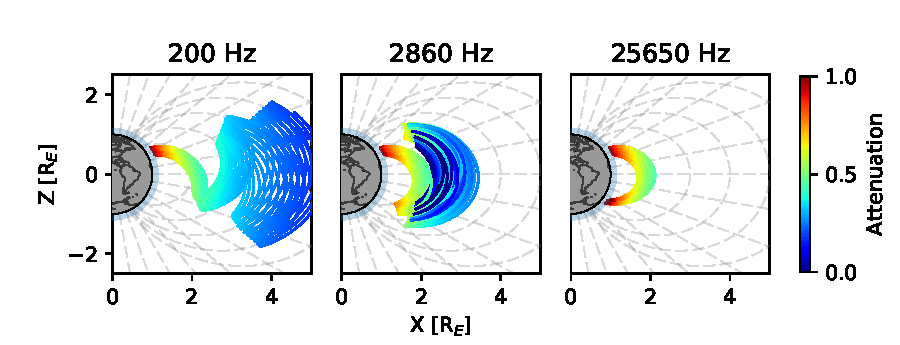
\includegraphics{Figures/raytracing_example.pdf}
\end{center}
\caption[Example ray tracing]{Example ray families as computed by the raytracer}
\end{figure}
\subsubsection{Adaptive Timestepping}
The process of raytracing, then, is to 1) solve the dispersion relation (\ref{eqn:disp_rln}) to find the refractive index; 2) compute the velocity vector and step the system forward in time; and 3) re-evaluate at the new position to assure that the condition F=0 is satisfied. However, properly selecting the timestep is of critical importance -- too large a timestep and positional errors will accumulate, or the ray will slip out of a propagating mode; too small and computational speed and memory usage suffers. We use an adaptive \emph{Runge-Kutta-Fehlberg} (RK45) \citep{Fehlberg1969, Mathews2004} method to continuously update the timestep as the raytracer progresses. RK45 is a common technique for solving ordinary differential equations.

The RK45 method approximates a solution with an initial stepsize $dt$ using two spline fits: a fourth-order and a fifth-order. The error in the step is taken to be the difference between the two estimates. If the error is above a specified tolerance $\epsilon$, the stepsize is reduced and the evaluation is repeated. Additionally, if the error is below a specified tolerance ($\epsilon/10$ in our implementation), the stepsize is increased. The result is a variable time axis with finer resolution in regions of high variability, while enabling longer timesteps in smooth regions for computational efficiency. See appendix \ref{appendix:runge_kutta} for a detailed description of the Runge-Kutta method.

\subsection{Landau Damping}
\label{section:damping}
The cold-plasma formulation of raytracing described above evaluates the trajectory and wavenormal angle of a wave packet. However, it assumes zero attenuation of wave energy. While it is possible to account for wave attenuation in ray tracing using warm plasma corrections \citep{Sazhin1993, Henyey1980}, we follow the same approximation as used in the legacy ray tracing code, and calculate attenuation along the cold-plasma raypath according to Landau damping.

Landau damping, originating in a seminal work by \cite{Landau1946}, is a resonant interaction between a wave and the distribution of electrons and ions comprising the background medium. The Landau mechanism is an interaction with parallel streaming particles and the wave's electric field. Resonant particles are accelerated or decelerated by the wave's electric field; if a majority of the resonant electrons have velocities slightly below that of the wave, then a coherent effect exists, the wavefront imparts some net energy to the plasma, and the wave is attenuated. Conversely, if the majority of resonant particles are moving faster than the wave, some of their energy can be imparted to the wavefront, inducing \emph{wave growth} \citep{Chen1983, Kulkarni2009}. 

Landau damping can have multiple resonances (in which the particle has multiple complete rotations per rotation of the wave). The lowest resonant mode is known as the \emph{Landau} resonance, while the $\pm 1$ modes are referred to as the \emph{Cyclotron} resonances. Higher-order modes remain nameless.

We use the expressions for Landau damping as formulated by \cite{Brinca1972}. \citeauthor{Brinca1972} derived expressions for Landau damping assuming a cold background plasma with a sparse warm distribution added, for Whistler waves propagating at an arbitrary angle to the background magnetic field. Inputs to this formulation are the familiar Stix parameters (equations \ref{eqn:stix_params_1} - \ref{eqn:stix_params_2}), which are in turn a function only of location and wave frequency; the wavenormal angle with respect to the background magnetic field; and a distribution function which specifies the energies (and thus velocities) of thermal electrons. The full set of Landau damping equations is given in appendix \ref{appendix:landau}.

Interestingly, \citeauthor{Brinca1972}'s work was motivated by measurements of Whistler-mode wave growth, rather than attenuation. Our implementation follows suit, and is equally capable of returning growth or damping, depending on the plasma model used. However, throughout this research, wave growth has been exceedingly rare.

\subsubsection{Thermal electron distributions}
\label{section:thermal_electron_distributions}
The extent to which a wave is amplified or damped is heavily dependent on the energy distribution of background electrons. The energy distribution, or temperature profile, is specified as a normalized function in phase space -- a function of position and velocity, which is normalized to 1:

\begin{eqnarray}
f  & = & f(\vec{r}, \vec{v}, t) \\
& =  & f(\vec{r}, v_\perp, v_\parallel, t) \\
\int_0^\infty f d v_\perp & = & 1 \\
\end{eqnarray}

Two distribution functions are used in similar work -- the \cite{Bell2002} distribution, which was derived from POLAR spacecraft measurements of the inner plasmasphere, and the \cite{Bortnik2007} distribution, which is based on CRRES spacecraft measurements above L $\approx$ 7.

We use the phase space density function as described in \cite{Golden2010}, which smoothly transitions between the \cite{Bell2002} model inside the plasmapause, and the \cite{Bortnik2007} model outside the plasmapause. Figure \ref{fig:phase_space_density} shows an example of the distribution function.

\begin{figure}[ht]
\begin{center}
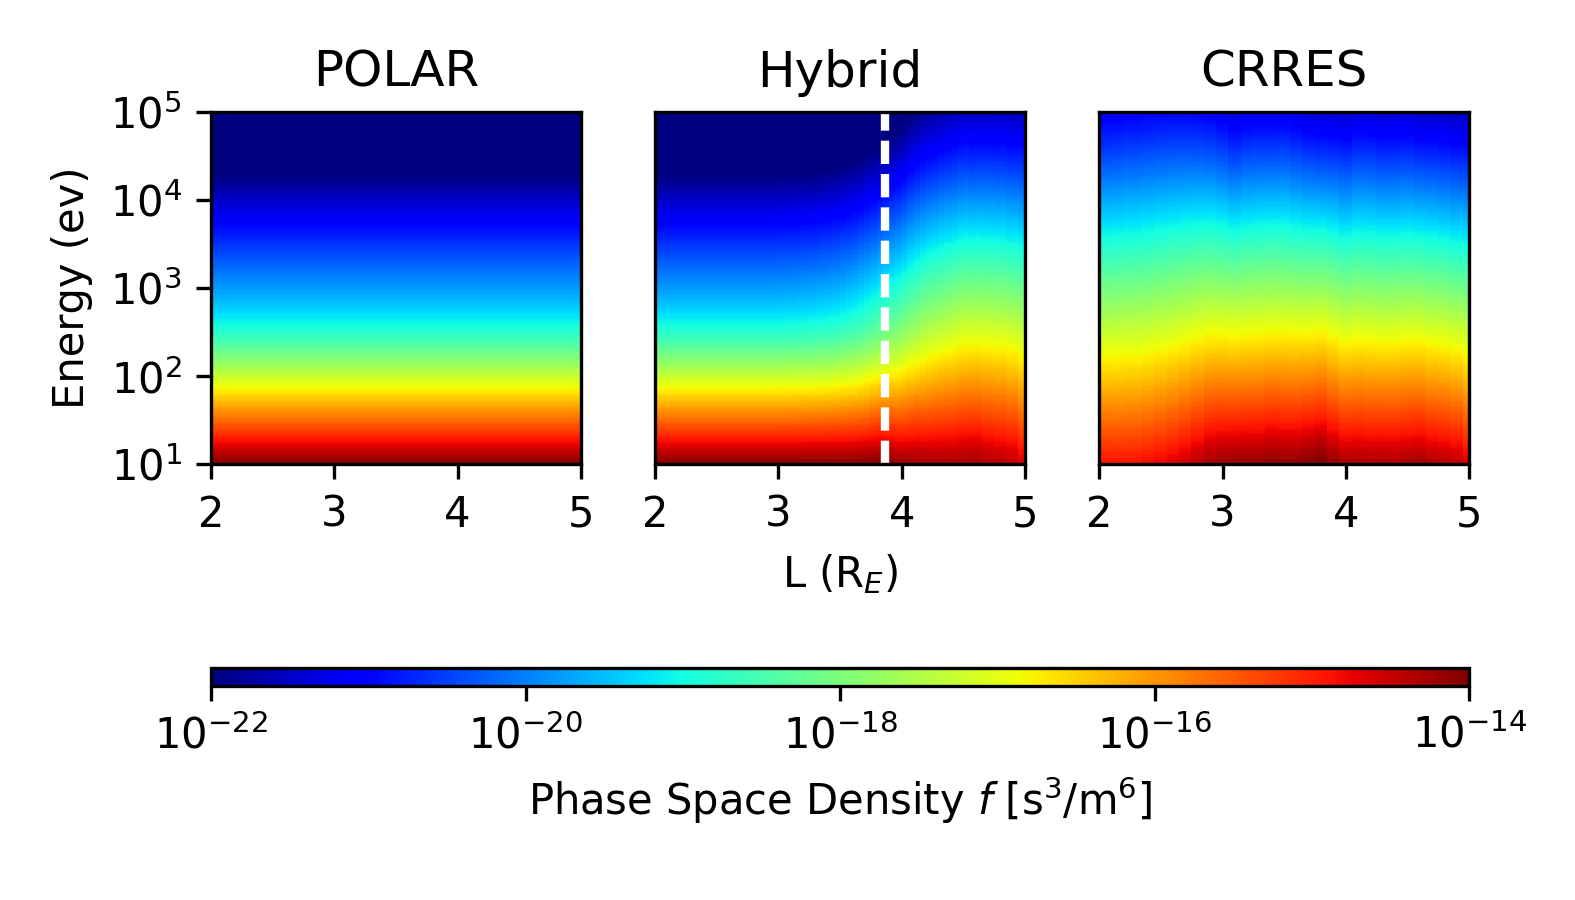
\includegraphics{Figures/psd.png}
\end{center}
\caption[Phase-space density functions]{Example phase-space density functions, shown for $A_e$=1.6, $K_p$=4, $\alpha$=45$^\circ$, and MLT=18. The POLAR model is used inside the plasmapause, and the CRRES model outside the plasmapause. The hybrid model smoothly transitions between the two. The plasmapause, at $L\approx 4$, is marked by the dashed white line.}
\label{fig:phase_space_density}
\end{figure}







